\section{Software}
Both the Assembler and the Programmer are C\# console applications developed in Visual Studio.\\ 
The code highlighter is a Node-JS Visual Studio Code Extension project developed in VS Code. 

\subsection{Assembler}
The HTMega Assembler read HTMega instructions from a .hasm or .asm file and assembles them into bytecode inside a .hex or .bin file.

\subsubsection{Running the Assembler}
The Assembler has to be called over console with up to two arguments:
\begin{mdframed}[backgroundcolor=light-gray, roundcorner=10pt,leftmargin=1, rightmargin=1, innerleftmargin=15, innertopmargin=6,innerbottommargin=6, outerlinewidth=1, linecolor=light-gray]
    \begin{lstlisting}[style=hasm]
    > HTMegaAssembler.exe <input .hasm/.asm> <(optional) output .hex/.bin>
    \end{lstlisting}
\end{mdframed}
If the second argument is omitted, the resulting output hex file will be placed next to the input file with the same name and the .hex extension.

\subsubsection{Errors}
The following additional errors are implemented:
\begin{itemize}
    \item Argument Error: 
    \begin{itemize}
        \item Wrong amount of arguments
        \item Argument not in path format 
        \item Input file does not exist 
        \item Wrong extension
    \end{itemize}
    \item Syntax Error:
    \begin{itemize}
        \item Invalid Mnemonic
        \item Wrong amount of parameters
    \end{itemize}
    \item Value Error:
    \begin{itemize}
        \item Parameter not of type uint8 (register address), uint16 (PM/RAM address)\\
            or int16 (immediate value)
        \item PM address exceeds address range of 50000
    \end{itemize}
\end{itemize}
\newpage


\subsubsection{Flow Chart}
\begin{figure}[h]
    \begin{center}
        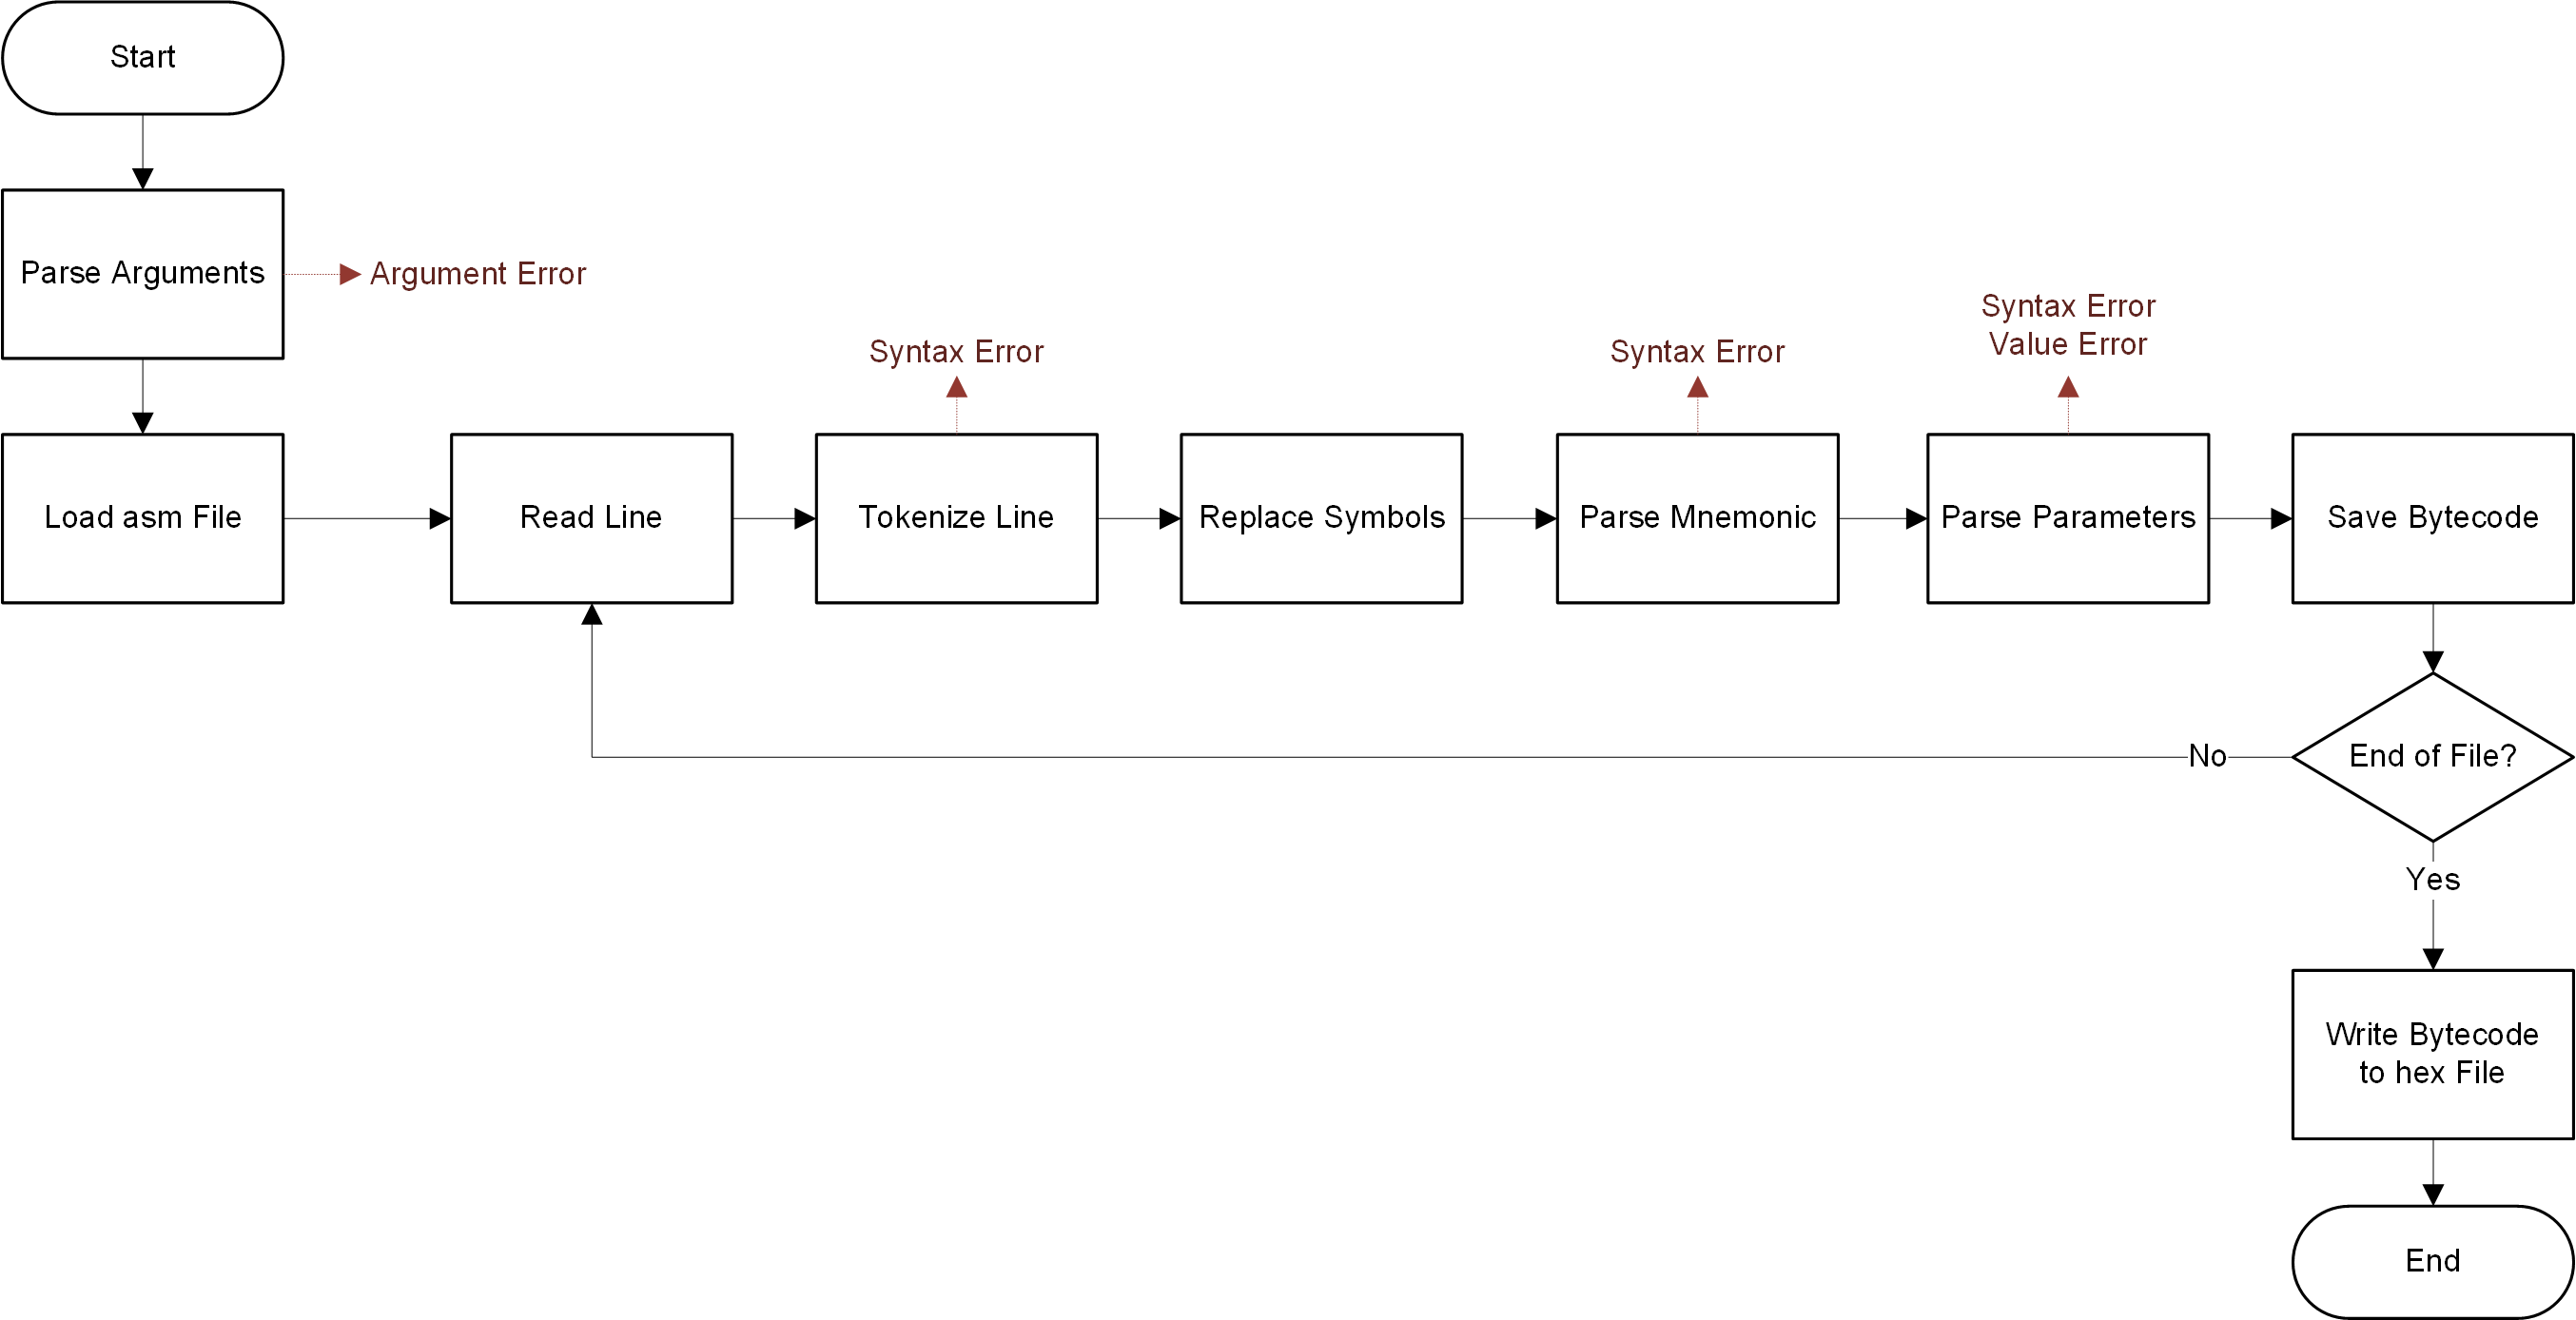
\includegraphics[scale=0.7]{assets/Assembler.png}
    \end{center}
    \caption{Assembler Flow Chart}
\end{figure}

\subsection{Programmer}
The HTMega Programmer reads a .hex or .bin file and sends the assembled program to the HTMega over USB.\\ 
The transmission to the HTMega begins with the start-byte 0xF1, followed by the bytecode.

\subsubsection{Running the Programmer}
The Programmer has to be called over console with up to two arguments:
\begin{mdframed}[backgroundcolor=light-gray, roundcorner=10pt,leftmargin=1, rightmargin=1, innerleftmargin=15, innertopmargin=6,innerbottommargin=6, outerlinewidth=1, linecolor=light-gray]
    \begin{lstlisting}[style=hasm]
    > HTMegaAssembler.exe <input .hex/.bin> <(optional) COM-Port>
    \end{lstlisting}
\end{mdframed}
If the second Argument is omitted, a selection with available COM-Ports will be shown.

\subsubsection{Errors}
The following errors are implemented, next to the C\# serial port exceptions \cite{serial-port-exceptions} :
\begin{itemize}
    \item Argument Error: 
    \begin{itemize}
        \item Wrong amount of arguments
        \item Argument not in path format 
        \item Input file does not exist 
        \item Wrong extension
        \item COM-Port does not exist or is not available
    \end{itemize}
\end{itemize}

\subsection{Code Highlighter}
VS Code syntax highlighting \cite{vscode-syntax} is powered by TextMate Grammar \cite{textmate-grammar} and uses regular expressions to select certain text.
The HTMega .hasm highlighter for consists of a tmLanguage.json file that includes the code highlighting configuration.\\

\paragraph{Example - Regular Expression to select literals:}
\begin{mdframed}[backgroundcolor=light-gray, roundcorner=10pt,leftmargin=1, rightmargin=1, innerleftmargin=15, innertopmargin=6,innerbottommargin=6, outerlinewidth=1, linecolor=light-gray]
\begin{lstlisting}[style=hasm]
(?i)\\b(([0-9]+)|(0x[0-9a-f]*)|(0b[01]*))\\b
\end{lstlisting}
\end{mdframed}
A list of regular expressions can be found in \cite{textmate-regex} - \citetitle{textmate-regex}.